\chapter{引言}
\section{研究背景和研究意义}
\subsection{研究背景}
自从十九世纪八十年代人类世界的第一辆汽车诞生以来,人类的生活就再也离不开汽车这种
方便的交通工具。尤其是进入21世纪以来,中国大陆地区汽车保有量快速上升,几乎到了家
家都有车的地步,一些富裕一些的家庭甚至一人一辆车。据不完全统计,在2002年左右我国
的汽车保有量在2000万辆左右,而到了2015年则增加到1.72亿辆之多,并且以每年百分之十
的速度持续增长。如此大量的汽车,在给我们带来诸多便利的同事,也增加了城市道路的
复旦和交通事故的发生率。如今,道路拥堵、违规停车、交通事故已成为每个城市管理者的
心头病。因此,各国政府也在一直不停的研究如何对车辆有效监管,提高道路利用率,避免
交通事故。在此前提下,诞生了两大热门研究方向:智能交通系统(Intelligent
Transportation System, ITS)和自动驾驶系统。这两项技术都旨在通过计算机技术来解决
交通管理等问题。而这两项技术中必不可少的一环便是进行车牌识别,即通过计算机视觉技
术,对图像(或视频)中的车牌进行准确的定位、分割和识别。

\subsection{研究意义}
从研究背景中我们可以知道,VLPR技术在实际生活中有着十分重要且广泛的应用。下面我们
举出几个实际生活中自动车牌识别系统的典型应用:

(1) 停车场的智能管理
一般而言,在住宅小区、大型商场、车站等地方都会建设配套的停车场。而如何对进出停车
场的车辆进行管理,则是一个十分重要的问题。目前常见的有三种方式:
\begin{itemize}
\item 纯人力管理
\item 发放出入门禁卡
\item 智能的电子化管理
\end{itemize}
其中前两种方式都有着管理成本高、需要人力维护等缺点,而通过使用智能化电子管理系统,
不仅有效降低了管理、维护成本,而且可以实现无人值守式停车场。因此可以看到目前使用
智能化电子管理的停车场数量在不断增加。一般的智能化电子管理系统是在停车场的出入口
架设摄像头,自动对进出的车辆进行拍照,并对车辆的车牌号进行识别,从而对车辆进行登
记管理。

(2) 停车场自动找车系统
随着停车场越建越大,相信在若大的停车场里找寻自己的车辆是每个车主都头疼过得问题。
目前市面上出现了一项新的自动找车系统,即通过在停车场内部署的大量摄像头,对停在不
同车位的车辆进行车牌识别。车主在找车的时候,只需在终端机上输入自己车辆的车牌号,
系统就会自动找到车辆位置,并为车主提供导航。这项技术也大大方便了人们的生活、提高
了停车场的用户体验。

(3) 电子警察系统
目前的电子警察系统,通过大量安装道路路口、路段上的摄像头,对车道内的机动车驾驶行
为进行不间断自动检测和记录,并检测车辆的违法驾驶行为。而这项系统也必然少不了车牌
识别系统的帮助。可以看到,目前通过对城市道路电子警察的大量部署,可以有效对城市道
路上的车辆进行24小时的监控,很大程度上降低了交通事故的发生率。

(4) 行车记录系统
随车道路上车辆的不断增加,交通事故总是不可避免。为了方便在发生事故时进行责任认定,
许多车主都在汽车上加装了行车记录仪以记录行车情况。而如果一个行车记录仪能够自动进
行车牌识别并记录行车过程中周围的车辆信息,则无疑会大大方便车主和交警进行事故责任
认定等。

(5) 自动驾驶系统
基于人工智能技术的自动驾驶系统被认为是未来交通系统的希望之星。众所周知,人类驾驶
员在驾驶过程中难免存在疲劳、注意力分散、视角盲区等问题,从而造成了大量的交通事故。
而自动驾驶系统则无这些缺陷,因此可以在很多情况下降低交通事故的发生概率。因此许多
科技公司和研究机构都投入了大量的人力物力以进行自动驾驶技术的研究。事实上德国已经
开始尝试使用自动驾驶的卡车进行高速公路货运,以减少人力成本和交通事故。因此,车牌
识别系统作为自动驾驶系统里必不可少的一个子环节,有着十分重要的研究意义。

\begin{figure}[ht]
  \centering
  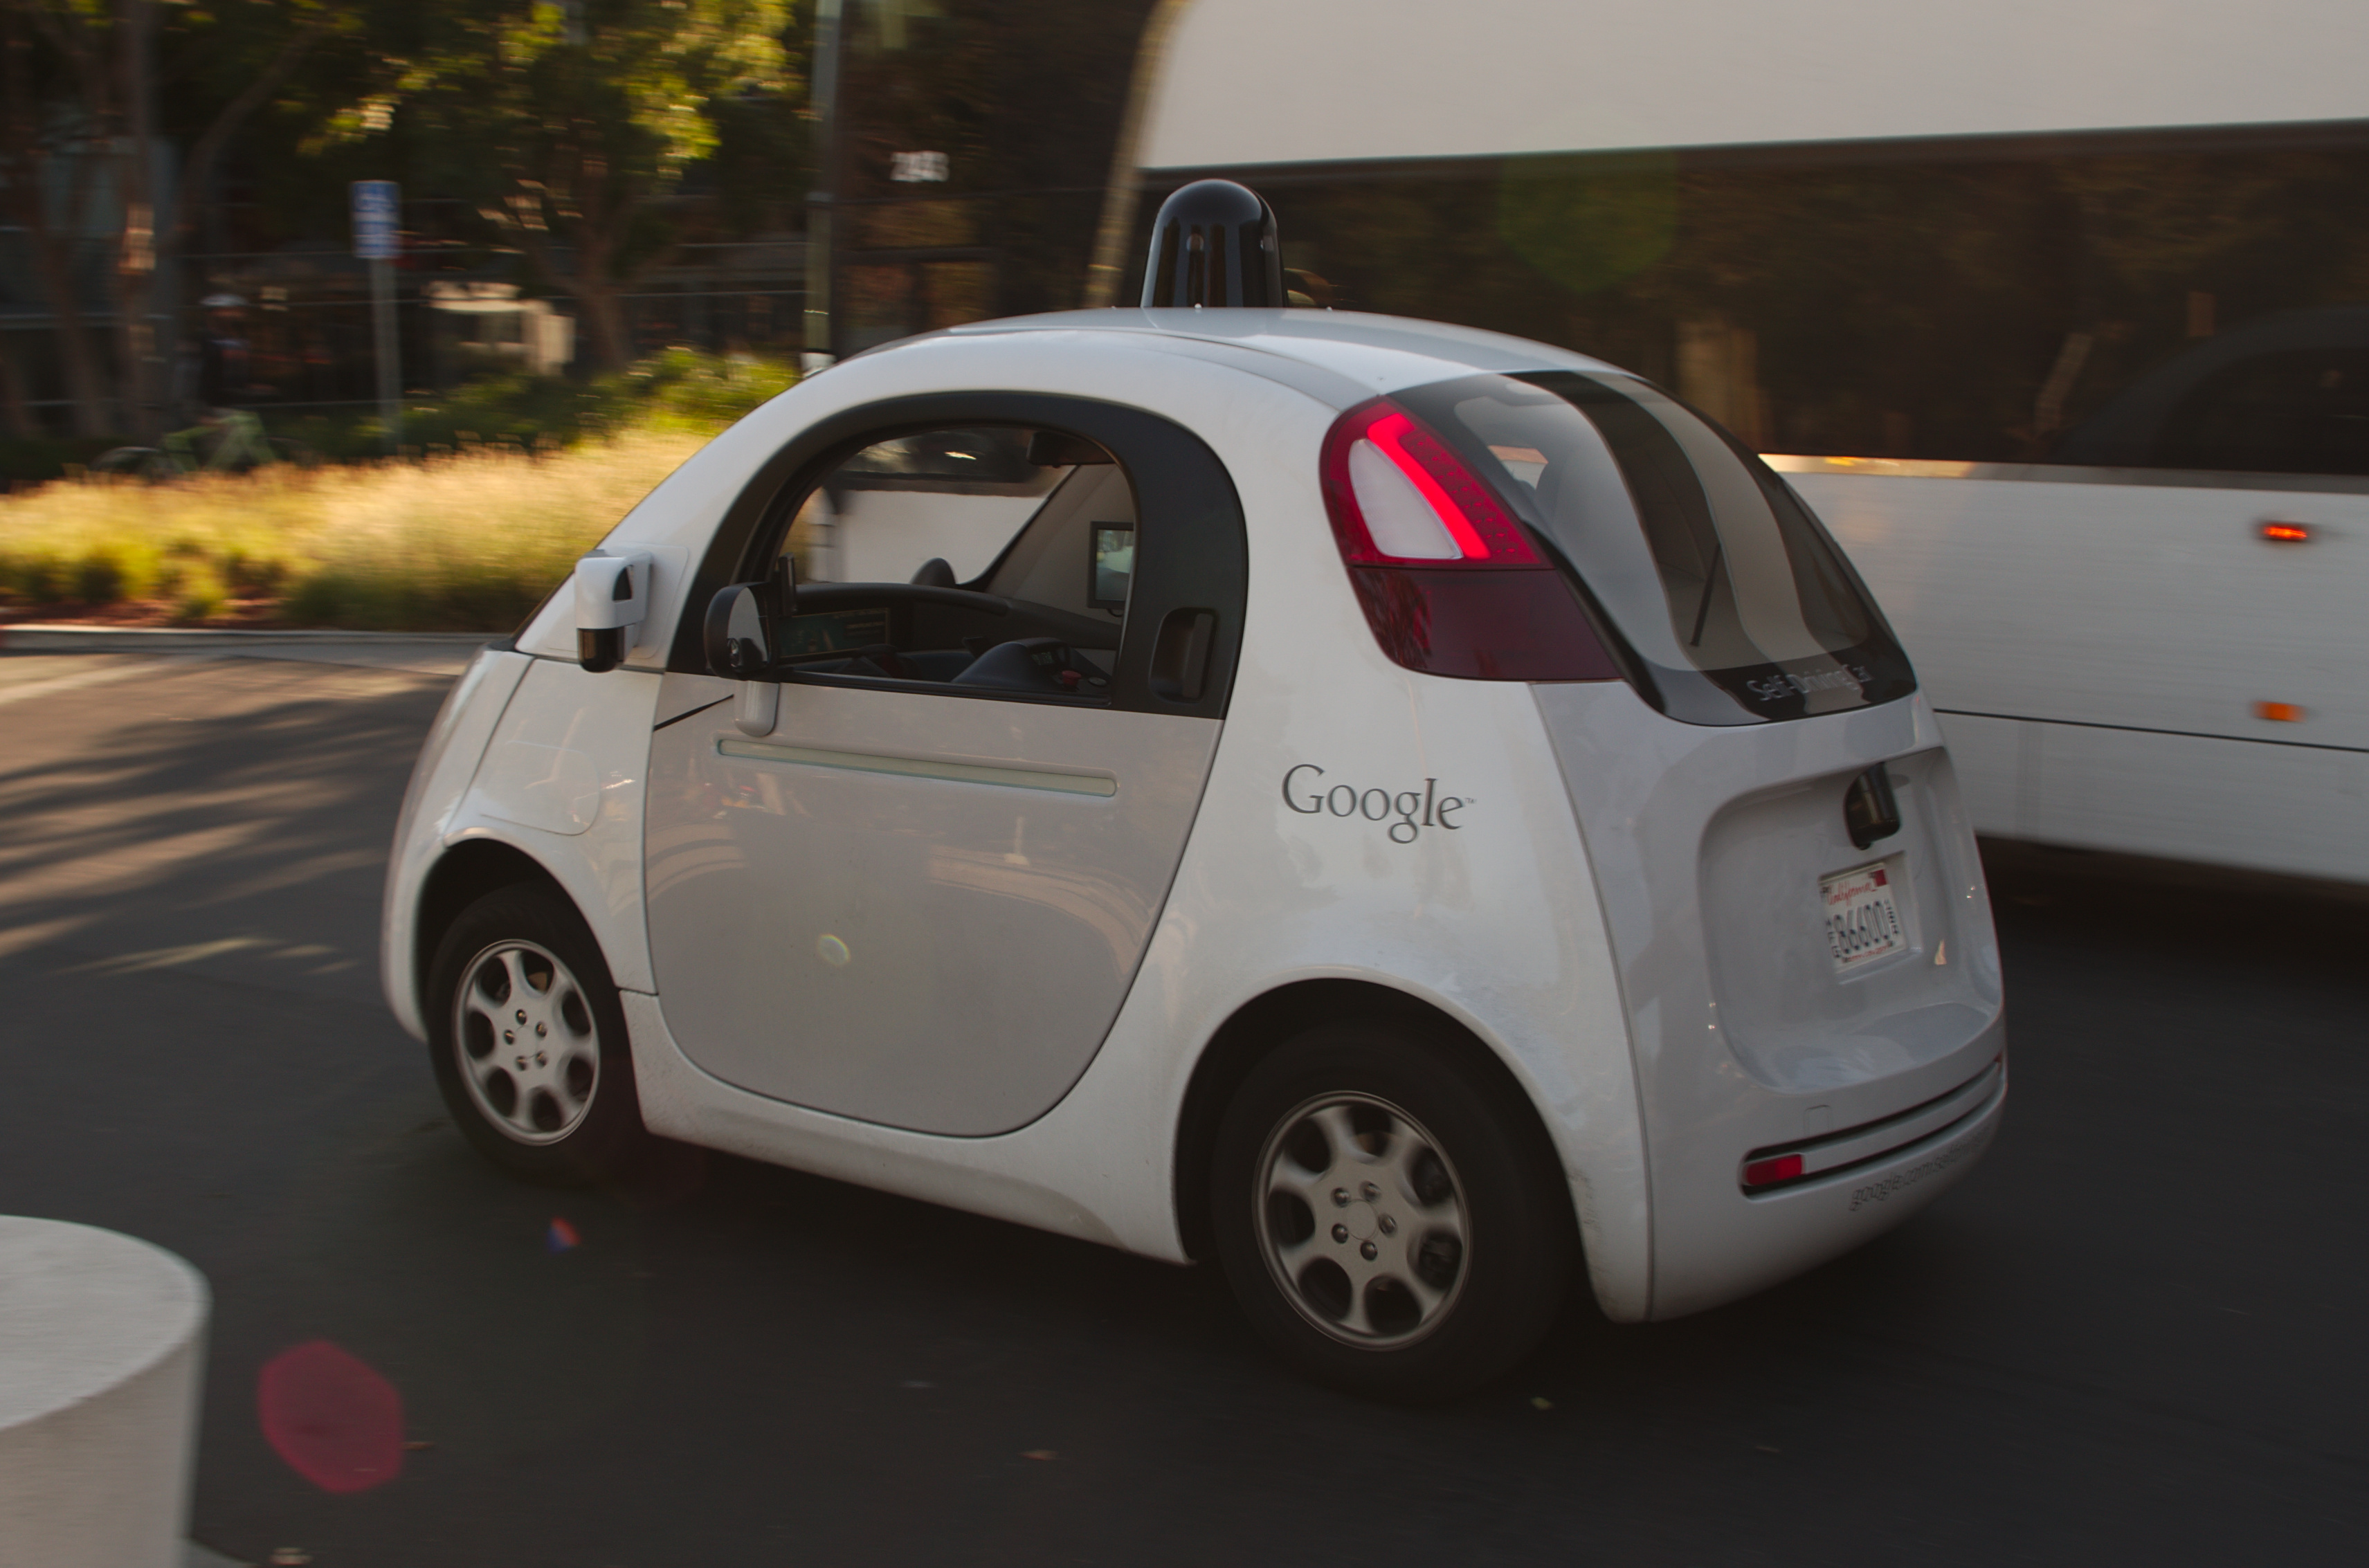
\includegraphics[width=0.8\linewidth]{./Figure/GoogleSelfDrivingCar.jpp}
  \caption{Google公司研制的无人驾驶汽车}
\end{figure}

综上所述,基于计算机视觉技术的车牌识别方法在诸多领域都有着极为广泛的应用前景和市
场价值,能够对社会和人类带来极为深远的影响。

\section{深度学习与计算机视觉}
\subsection{传统方法}
本文中提到的传统方法,是指在机器学习技术引入计算机视觉之前,人们为了解决常见的视
觉问题发明的大量基于手工特征和手工规则的方法。比较经典的,比如用于直线、曲线检测的
广义Hough变换\cite{Duda:1972eu},用于边缘检测的Sobel算子以及
SIFT\cite{Lowe:2004kd}、SURF\cite{Baya:2008ud}等图像特征。这些方法在早期的计
算机视觉任务中被大量的使用,并取得了一定的效果。比如,许多车牌检测系统使用Hough变
换对车牌的边缘进行检测从而实现车牌边缘的定位;使用二值化方法结合直方图投影进行车
牌字符分割。
由于传统的计算机视觉方法严重依赖于图像特征的选择,因此这些方法不仅需要花费大量的
精力进行特征工程,而且难以胜任一些复杂的计算机视觉任务,比如自然场景中的物体检测、
字符识别等任务。同时,即使是在一些已取得成功应用的领域,这些方法的效果也与人类视
觉系统的能力相距甚远。于是很自然的,人们就想如果手工设定的规则和特征不能很好的适
用于各种复杂计算机视觉任务,那为什么不让计算机自己从数据中学习特征和规则呢?于是
机器学习技术开始被应用于计算机视觉任务中,其中在近几年的研究中又以深度学习技术效
果最好、应用最广。


\subsection{深度学习}
所谓深度学习技术,实际上就是神经网络技术,只不过相较于传统的多层感知机等浅层神经
网络模型,深度学习中使用的网络模型层数更多(即更深)、规模更大。目前主流的深度神
经网络模型可以分为卷积神经网络CNN和递归神经网路RNN 两类。其中CNN 被广泛应用于各类
图像相关的计算机视觉任务中,而RNN 更多的应用在自然语言处理、时间序列预测等时序相
关的任务中。本文所采用的方法都是基于CNN 的,因此在此着重介绍CNN 的发展和应用。
1998年前后,Yann LeCun教授第一次成功将CNN 技术应用于手写数字识别任务
\cite{LeCun:1990vp},并取得了与人类水平相当的准确率。这一成果被直接应用于许多支票识
别系统系统中。但随后由于人工智能的第二次低潮,CNN 技术的研究一直进展缓慢。不过随
着摩尔定律导致的计算能力提升和互联网带来的海量数据,在2012年前后,Hinton 等人
使用深度神经网络技术在ImageNet 比赛中以准确率高出第二名百分之二十的惊艳成绩夺得第
一名\cite{Krizhevsky:2012wl}。值得注意的是,2012年ImageNet 比赛中第二名所使用的方
法正是基于复杂特征工程和统计机器学习的“传统方法”,因此这次事件揭示出在面对计算机
视觉任务时相较于传统方法的巨大潜力与优势。值得一提的是,自2012年以后,ImageNet 每
年的第一名都是深度学习方法,比如2015年的第一名是由Kaiming He等人发明的Residual
Network\cite{He:2015tt}。
相较于传统方法,CNN 最大的特点在于,它可以自动从数据集中学习图像特征,而不需要依
赖复杂的特征工程。实践证明,通过CNN 学习出来的特征,在许多计算机复杂视觉任务中要优于
通过特征工程设计的手工特征。同时,许多研究也表明,人类的视觉系统有着与CNN 相似的
结构,这似乎也解释了为何在复杂计算机视觉任务中CNN 可以取得和人类视觉系统相当的水
平。目前,除了字符识别、图像识别等任务外,深度学习技术也被成功应用于物体检测、图像语
义分割、图像标注等任务中。
但另一方面,由于关于神经网络人们还未能建立一个精确地数学模型来描述其特性和行为,
神经网络作为一个难以解释的“黑箱”一直饱受统计学派机器学习研究者的诟病。不过相信随
着研究的深入,这些问题在未来都可以得到解决。

\section{本文的内容安排}

一般的车牌识别系统主要分为如下几步进行:

\begin{enumerate}
\item 图像采集
\item 图像预处理
\item 车牌检测
\item 车牌精确定位
\item 车牌字符分割
\item 车牌字符识别
\end{enumerate}

其中,车牌检测、车牌精确定位、车牌字符分割和车牌字符识别则是整个系统的核心和难点,
本文也着重对这四个子问题进行分析研究。

本文的内容安排如下:

第一章,为引言内容。介绍了课题研究的背景和意义。
第二章,为车牌精确定位方法研究。这一章首先介绍了CNN 的基本概念和原理,然后阐述如
何使用CNN 进行关键点回归以进行车牌的精确定位
第三章,为车牌的检测方法研究。这一章首先介绍了Region CNN(RCNN)系列技术,包括
RCNN、Fast RCNN和Faster RCNN。然后通过Faster RCNN 技术实现了自然场景中车牌的检测。
第四章,为车牌字符分割方法方法研究。本章首先介绍了几种传统的车牌分割方法,并分析
了他们的优缺点。然后本章提出一种新的基于Extremal Region的方法进行车牌字符分割。
第五章,为车牌识别方法的研究。本章阐述如何通过卷积神经网络(CNN)技术进行车牌字
符识别,并进行相关实验。
第六章,为总结和展望。总结了本文的主要工作,并对未来的研究做了简单的介绍。

\section{本章小结}
本章从车牌识别的研究背景和研究意义展开讨论,说明了本研究的意义和价值;然后简要介
绍了两种研究思路——即传统方法和深度学习技术;最后简要说明了本文的内容安排。

\chapter{车牌精确定位}

在许多未使用深度学习技术的车牌识别系统中,倾向于使用边缘检测、Hough变换等寻找车
牌的边缘与顶点,直接实现车牌的检测与精确定位,但这些传统方法有着对图像质量、背景
颜色敏感,抗噪声能力差,难以处理特殊情况等诸多缺点,在很大程度上限制了其应用。因
此在本文中我们将车牌的定位分为车牌检测与车牌精确定位两步进行。其中车牌检测用于找
到图像中包含整个车牌的小区域,然后车牌精确定位则从这个小区域中找寻车牌的四个顶点
以进行精确定位。关于车牌检测技术将在本文第三章进行介绍,本章将介绍如何使用CNN 技
术进行车牌精确定位。在本章内容中,我们将车牌精确定位问题视为一个回归问题,然后讨
论如何使用CNN 对关键点进行回归的以实现精确定位,并进行实验验证。

\section{卷积神经网络概述}

卷积神经网络是一种前馈神经网络,一般有许多个卷积层和顶端的全连接层(对应经典的多
层感知机)组成,同时也包括相应的权重和池化层(Pooling Layer)。这一结构是的卷积
神经网络能够有效利用输入数据的二维结构,同时还极大程度减少了网络参数,降低了训练
难度和过拟合的风险。因此卷积神经网络在图像检测、识别方面取得了非常有优异的结构。
如2015年微软亚洲研究院Kaiming He等人发明的Residual Network成功的将ImageNet Top-5
错误率降低到了5\%左右\cite{He:2015tt}\cite{He:2016tq}。

\begin{figure}[ht]
  \centering
  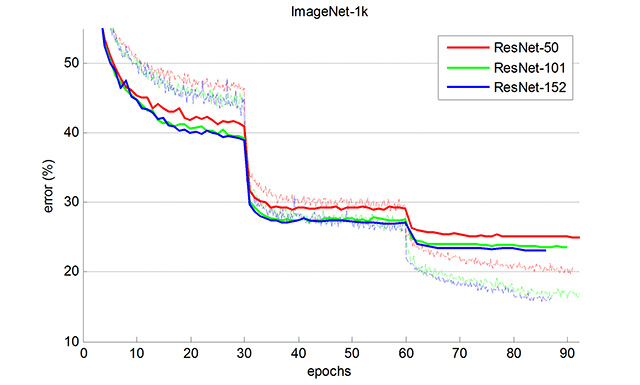
\includegraphics[width=0.8/linewidth]{./Figure/ResNetTrainError.jpg}
  \caption{Residual Network训练误差曲线\cite{He:2015tt}}
\end{figure}

\subsection{卷积层}

所谓卷积层,是指使用一个相对较小的卷积核(Kernel)在整幅图像上滑动并进行卷积操作
并通过非线性激活函数从而得到输出的一种特殊的神经网络结构。常见的卷积核大小有 $1
\times 1, 3 \times 3, 5 \times 5, 7 \times 7$ 等。可以看到,卷积层的参数要远远少
于输入输出大小的全连接层,参数的减少不仅极大程度降低了网络的训练难度,而且有效避
免了过拟合的出现。一般一个卷积层会有多个卷积核,每一个卷积核可以提取图像的不同特
征,从而得到不同的特征映射。图 \ref{Fig: LeNet} 是LeNet\cite{LeCun:1990vp}的网络
结构。

\begin{figure}[ht]
  \centering
  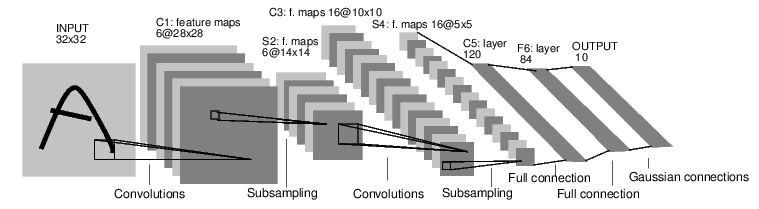
\includegraphics[width=0.8/linewidth]{./Figure/LeNet.png}
  \caption{用于手写数字识别的LeNet5\cite{LeCun:1990vp}} \label{Fig:LeNet}
\end{figure}

\subsection{池化层}

很多情况下,使用卷积得到的特征映射尺寸仍旧很大,为了进一步减少网络参数,从而降低
训练难度和过拟合的风险,经常在网络中加入一些池化层。池化层没有内在参数,仅仅是对
卷记得到的特征映射在不同位置进行聚合统计(如取平均值、取极大值等)。

\section{使用卷积神经网络进行车牌精确定位}

\subsection{数据处理}

在本文的实现中,我们首先将待处理的图片统一缩放至 $448 \times 224$ 的分辨率,并进
行零化和标准化操作,图像色彩空间选择为RGB 色彩空间。
此外,由于卷积神经网路不具有仿射不变性,因此我们需要对训练集进行数据扩张(Data
Augmentation),具体来讲就是对图片进行随机的旋转和放缩,从而增加CNN 抵抗仿射变换
的能力。

\subsection{模型设计}

车牌的精确定位问题可以看作一个对车牌四个顶点坐标进行回归的回归问题,因此我们可以
很容易的通过卷积神经网络搭建这样一个回归模型,其输入是经过缩放的车牌区域图片,输
出则是车牌四个顶点的坐标。本文并未从头训练一个全新的模型完成此任务,而是使用一个
训练好的模型,保留其卷积部分并将以Softmax 为激活函数的分类层更换为无激活函数的回
归层。具体来讲本文中使用的是训练好的34层Residual Network模型。

\subsection{实现环境}

本章的神经网络使用Torch 7框架进行实现,实验机器配置如下:

\begin{tabular}{|c|c|}
\hline
项目 & 规格说明 \\
操作系统 & Ubuntu Server 14.04
\hline
CPU & Intel \\
\hline
内存 & 32GB DDR3 \\
\hline
显卡 & NVIDIA Quardo M5000 x2 \\
\hline
\end{tabular}

训练数据集大小为900张,测试数据集为100张,训练使用参数如下:


\subsection{实验结果与分析}

训练loss曲线
测试集上Mean Error和Max Error的曲线

结果图

可以看出,使用CNN 进行车牌精确定位可以较为有效的进行车牌定位,而且不需要手工选择
特征,鲁棒性强。但另一方面,由于神经网络的训练由于不需要先验知识,导致其对数据质
量和数量要求很高,而能否获取大量带标注的车牌数据进行训练,将直接影响这一步的结果。
相信如果能获得更大的带标注训练数据集,本算法的效果还有进一步提升的空间。

\section{本章小结}

本章主要简要介绍了CNN 的基本概念,然后基于34层的Residual Network设计了一个用于实现
车牌精确定位的卷积神经网络回归模型,并通过实验验证了其效果,证明了本方法的可行性。
最后提出通过增加训练数据集的大小,可以进一步提高模型的精度和效果。

\chapter{车牌检测}

所谓车牌检测,即是从一幅图像中找寻包含车牌的子图像,显然这属于目标检测(Object
Detection)问题。目标检测技术作为一个十分热门的研究领域,经历了从十年前HoG 方法大
行其道到如今RCNN 技术一统天下的发展过程。RCNN 技术于20xx年由xxx提出,随后又出现
了Fast RCNN和Faster RCNN 两代的改进。如今, Faster RCNN 技术不仅在Pascal VOC和
COCO 两个数据集上的目标检测任务中取得了最佳的效果,而且在借助GPU 加速的情况下做
到实时检测(0.2s/帧)。因此本章将首先简要介绍RCNN 系列技术,然后在我们的数据集上
对其效果进行试验验证。
 '
\section{Region CNN 概述}

\subsection{RCNN}

\subsection{Fast RCNN}

\subsection{Faster RCNN}

\section{使用Faster RCNN进行车牌检测}

\subsection{数据集准备}

(1) 车牌图片
本文选择了1000张在道路上拍摄的含有车牌的照片,注意这些照片为步行或行车过程中使用
手机拍摄而来。

(2) 数据标注
本文中首先对这些车牌的四个顶点进行手工标注,然后取包含车牌区域的最小外接矩形作为
ground truth用于Faster RCNN 的训练。

\subsection{实现环境}

本文的Faster RCNN 实现基于开源项目 py-faster-rcnn
\footnote{https://github.com/rbgirshick/py-faster-rcnn.git}修改而来,增加了对上
一步构造出的车牌数据的支持。

训练网络使用的工作站配置如下:

\begin{tabular}{|c|c|}
\hline
项目 & 规格说明 \\
操作系统 & Ubuntu Server 14.04
\hline
CPU & Intel \\
\hline
内存 & 32GB DDR3 \\
\hline
显卡 & NVIDIA Quardo M5000 x2 \\
\hline
\end{tabular}

训练数据集图片为900张,测试数据集图片为100张,模型参数为如下:

\subsection{实验结果与分析}

经过训练,Faster RCNN在100张测试数据集上精度达到84.54\%,相信如果换用更大的训练
数据集后效果还可进一步提升。

识别举例图

\section{本章小结}

本章首先介绍了使用RCNN 系列算法进行物体检测的基本原理,然后通过修改开源项目
py-faster-rcnn,在我们的车牌数据集上进行训练,最后验证其识别准确率可以达到85\%左
右,验证了使用Faster RCNN 进行车牌检测的有效性。

\chapter{车牌字符分割}

\section{Extremal Region}

\section{使用Class-specific Extremal Region进行车牌字符分割}

\subsection{算法实现}

\subsection{本章小结}

\chapter{车牌字符识别}

\section{使用CNN进行车牌字符识别}

\subsection{模型设计}

\subsection{实验结果}

\section{本章小结}

\chapter{总结与展望}

\section{总结}

自从2006年Hinton 带领神经网络学派以深度学习的新名字复苏以来,深度学习由于其令人
惊艳的性能和易于使用等特点,无论是在学术界还是在工业界都有着十分广泛的应用。今年
三月Google DeepMind 团队开发的AlphaGo 以4:0的优秀成绩大败人类围棋冠军李世乭轰动
世界,而深度学习、人工智能等名词常见于各种媒体平台,称为当之无愧的流行用语。此外,
无论是金融圈还是IT业,都有无数的公司投入大量的资金和人力进行深度学习、人工智能的
研究,毋庸置疑,机器学习技术,尤其是深度学习技术已成为时下最热门的研究领域。
不仅如此,深度学习技术也在潜移默化间改变着我们的生活。小到越来越准确的语音识别技
术、越来越贴合用户需求的搜索引擎、购物平台、音乐推荐系统等,大到可以下赢世界冠军
的AlphaGo 围棋程序,都离不开深度学习技术的助力,甚至连NVIDIA 公司也借卖显卡做深度
学习而发了财。可以预见,在不远的将来深度学习将像两次科技革命一样颠覆我们的生活,
造福人类社会。
本文试图将最新、最好的深度学习技术引入车牌识别这一任务中,从而实现更鲁棒、更智能
的车牌识别系统。具体来讲,有以下几点:
首先,本文试图使用Faster RCNN 这一目标检测神器来实现车牌的检测。基于Faster RCNN的
方法能有效克服传统方法不够鲁棒、依赖先验知识、特殊情况多等缺点,实现更加智能、更
加鲁棒的车牌定位系统。
再次,本文提出使用CNN 回归的方式对车牌坐标进行精确定位,从而抛弃传统的基于边缘检
测的方法,以提高性能的适应性。
然后,本文抛弃了传统的基于连通域和垂直投影的车牌分割方法,尝试将车牌字符分割变为
一个文字检测问题,并通过Class-specific Extremal Region的方法进行解决,有效克服了
两种传统方法的缺点。
最后,本文使用CNN 技术进行车牌字符识别,获得了极高的准确率。将中文字符和英文数字
分开训练的做法更是增加了识别的准确率和可靠性。

\section{展望}

本文虽然使用深度学习技术进行车牌识别,克服了传统方法的诸多缺点,但也可以看到深度
学习方法也不是完美的,甚至在很多应用场景下性价比不如传统方法高。展望未来工作,我
希望从以下几个方面对整个系统进行改进:

第一,Faster RCNN 技术虽然在目标检测问题上表现优异,但其速度仍旧偏慢,不能很好地
适用于高速公路等对检测速度要求高的场合。而近年流行的另一种基于CNN 的目标检测技
术——You Only Look Once——简称YOLO,虽然准确率不如Faster RCNN,却有着非常快的速度,
因此可以考虑使用YOLO代替Faster RCNN 技术进行车牌目标检测。
第二,在车牌字符分割过程中,我们需要去除大量假阳性的Extremal Region,目前我们采
用的方法是基于车牌字符的相对位置和尺寸进行筛选,但这种方法严重依赖先验知识和对筛
选规则的制定,造成了大量无法处理的特殊情况。因此我们希望通过机器学习技术完成ER的
合并工作,一种可行的思路是使用文献\cite{Gomez:2014vp}中的方法进行区域聚合,来同
时实现车牌文字区域的精确定位和分割。